\documentclass[12pt, a4paper]{article}
\usepackage[utf8]{inputenc}
\usepackage{graphicx}
\graphicspath{ {./desktop} }
\usepackage{indentfirst}
\usepackage{microtype}
\usepackage[breaklinks]{hyperref}
\setlength{\parskip}{1em} 
\begin{titlepage}
\title{Wearable Sensor App Manual}
\author{Bourdage, R., van Dijk, M. \& Gawhns, D.}

\date{Leiden Institute of Advance Computer Science

 June 2021}

\end{titlepage}



\begin{document}

\maketitle
\thispagestyle{empty} 
\newpage
\tableofcontents
\newpage
\cleardoublepage


\section{Introduction}

The ``liacs.sensorapplication" software was created for the Samsung Gear Fit Pro 2, which is a digital watch issued in 2016 containing an  accelerometer, gyroscope, barometer and GPS sensors.This Samsung wearable runs on Tizen OS version 2.3.1:13 and is based on Linux OS.The wearable sensor was selected for a research project as it's operating system allowed for the extraction of raw data files. In addition, the wearable had to be customizable to incorporate the following additional research project requirements: patient id, the recording of sensor files, saving of the measurement settings and privacy settings. Samsung offered Tizen Studio software environment free of charge to design applications and services for the watch. Many programming examples and API documentation were also available online.(see: https://developer.samsung.com/tizen/Galaxy-Watch /certificate/creating-certificate.html)

\cleardoublepage

\section{The Software Package}
The software package contains a Tizen OS widget application named  ``liacs.sensorapplication" visible in the list of applications with title ``Sensors" and a digital brain as icon. The application carries a snipper entry widget control to enter the person id, a number between 000 and 999, and two buttons; the RESTART button to start and restart measurements and the CLEAN button to be pressed 3x to remove all measurements from the watch.The activity data is stored in sensor files and have a file name which contains the person id, watch id, date, time and sensor type. The package is configured by a configuration file which is pushed on the watch in an application independent accessible file system folder. 



The configuration is stored for every measurement. The configuration file consists of: a) the recording in terms of frequency; b) recorded sensors; and c) the centre and size of the privacy circle. For reproducibility and data management, a naming convention was developed for all files, including the con files, listed in the following order: a) Patient ID; b) Watch ID; c) Date (YYYY, MM , DD); d) Time (HR, Minute, Seconds). For an example:


001 2021 05 13 10 44 00 d9a8 aag.dat


002 2021 05 12 11 09 09 d9d2 bar.dat


003 2021 05 13 10 43 01 d9d7 con.dat


004 2021 05 12 11 06 49 d9d6 gps.dat

For power consumption and memory size, the gravity accelerometer and gyroscope sensors with high frequency readouts are separately stored from the low frequency readouts of the barometer, battery charge percentage and GPS values. The sensor values are stored in a commonly used file format, the comma separated value file format.

\begin{center}
    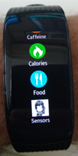
\includegraphics[width=.2\textwidth]{Pic 1.png}
    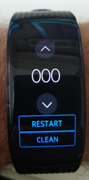
\includegraphics[width=.199\textwidth]{Pic 2.png}
\end{center}

The software package also contains a Tizen OS widget service named ``liacs.sensorservice" which runs in the background, not visible in the list of applications and cannot be deleted by the user of the watch. The sensor service processes the messages RESTART and CLEAN send by the sensor application. After the start of the watch, the sensor service is activated and waiting for these messages. After one valid message received, the service starts the recording of the sensor values and stores it into comma separated values files. The measurement is based on the contents of the uploaded configuration file. Wifi on the watch needs to be on when uploading the con file and to download the collected data off of the watch. Otherwise, wifi can be off during data collection. In addition, the watch's GPS needs to be turned on to collect GPS data.


A figure in Appendix A shows a state diagram with transitions and format ``event - actions", as a formal description of the states and relevant state events between the watch application manager, the sensor application and service.



The wearable was manually tested. The accelerometer and the gyroscope were validated by perpetually rotating the watch at different speeds. The barometer was validated by comparing height differences in a GPS track with the air pressure measured. Zero measurements were obtained by calculating accelerometer means and standard deviations and comparing the results between watches. The variance between watches was of 0.028 on average. In order to account for this variance, a threshold was created by using the following formula: threshold = mean(G) + 4 * std(G), where G = the gravity acceleration vector norm [sqrt( ax2 + ay2 + az**2)]. For reproducibility, it is advised to calibrate the sensor values and convert them to SI basic units before data processing. 


For a Python notebook, see Appendix B for calculating means and standard deviations and Appendix C for plots. Below, find sample of calculation outcomes. 



\begin{center}
    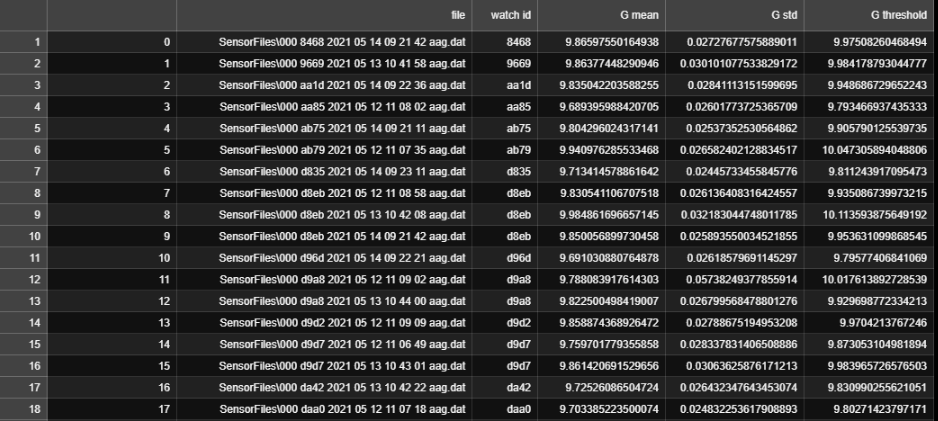
\includegraphics[width=.999\textwidth]{Pic 44.png}
\end{center}


For every sensor readout frequency, a separate sensor file is created. This reduces power
consumption and memory usage. The application contains a clock which
is used for all recordings so the data can be aligned with time. The
sensor values are stored in a commonly used file format, the comma
separated value file format.

The wearable chosen meets the requirements set out in 2018. 

\cleardoublepage
\section{How to use the Watch}
\begin{enumerate}
  \item Charge watch on charging dock
  \begin{center}
    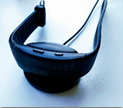
\includegraphics[width=.35\textwidth]{Pic 3.png}
\end{center}
  \item Switch on the watch after charging by pressing and holding small side button
    \begin{center}
    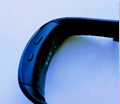
\includegraphics[width=.35\textwidth]{Pic 4.png}
\end{center}
  \item Access the Settings by pressing small side button once
    \begin{center}
    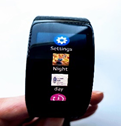
\includegraphics[width=.35\textwidth]{Pic 5.png}
\end{center}
\cleardoublepage
  \item Also found on the main screen is the Sensors app 
    \begin{center}
    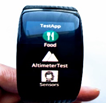
\includegraphics[width=.35\textwidth]{Pic 6.png}
\end{center}
  \item Press on the Sensor app, input an identifier and press restart to begin measurement. To delete any data collected, press Clean button three times  
    \begin{center}
    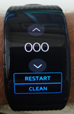
\includegraphics[width=.25\textwidth]{Pic 7.png}
\end{center}
  \item To turn off watch, press and hold small side button
    \begin{center}
    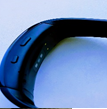
\includegraphics[width=.35\textwidth]{Pic 8.png}
\end{center}
\end{enumerate}
\cleardoublepage

\section{Installation of Tizen Studio Environment}

\begin{enumerate}
  \item Install Tizen Studio 4.1 with IDE installer. Once instillation is completed, the package manager will be prompted
  \item Install the Tizen extensions for native development for version 2.3.1 (tab: Main SDK). The watch has version 2.3.1:13 of the Tizen OS, therefore choose to install the 2.3.1 SDK together with the certificate SDK.
  \item Install the Tizen extension for Certificates (tab: Extension SDK)*
  \item Make a Samsung developer account, this will be required to create the necessary certificates: https://developer.samsung.com/sa/signIn.do 
  \item Run package manager (Tizen Studio - tools), go through the wizard steps.
\end{enumerate}

Note: Installation guide of the Tizen Studio development environment can be found in https://developer.samsung.com/tizen/Galaxy-Watch/certificate/creating-certificate.html 

\subsection{*More on Certificates}
\begin{enumerate}
  \item Connect watch via device manager (see How to Connect Watch to Tizen)
  \item Open Certificate Manager
  \item Hover over the little plus to add a new certificate
  \item Click Samsung Certificate
  \item You will be asked to make an author certificate and a distributor certificate
  \item If you want to add a watch: click on the plus sign as if adding a new certificate, click samsung certificate, select use existing certificate profile, click no when asked if you want to create a new author certificate, create new distributor certificate, you will be asked to chose a password and either add a DUID manually or connect to the new device. Alternatively, you can use a .txt file with a new DUID per line to create certificates.
\end{enumerate}
Tip: consider setting the date to one day in the future while setting up the watch to avoid certification date issues.

\section{How to Connect Watch to Tizen}
\begin{enumerate}
  \item To connect the watch to Tizen Studio, go to the computer’s ``Settings” window, navigate to the “Mobile Hotspot” and turn it on. It will then display a Network Name and Network Password
      \begin{center}
    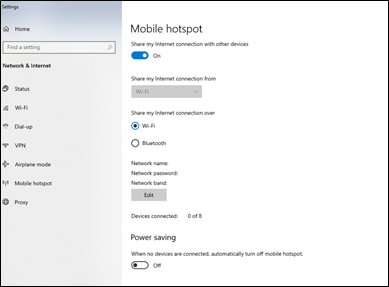
\includegraphics[width=.6\textwidth]{Pic 9.2.png}
\end{center}
  \item After the hotspot is turned on, go into the watches’ settings, and select the ``Connections"
      \begin{center}
    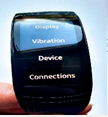
\includegraphics[width=.3\textwidth]{Pic 10.png}
\end{center}
\cleardoublepage
  \item Go to ``Wi-Fi" and turn it on
      \begin{center}
    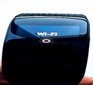
\includegraphics[width=.3\textwidth]{Pic 11.png}
\end{center}
  \item Press on ``Wi-Fi Networks" and select the laptop's mobile hotspot
      \begin{center}
    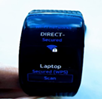
\includegraphics[width=.3\textwidth]{Pic 12.png}
\end{center}
  \item Press on ``Password" to enter the laptop's password
      \begin{center}
    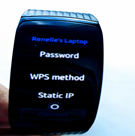
\includegraphics[width=.3\textwidth]{Pic 13.png}
\end{center}
\cleardoublepage
  \item Make sure that the watch has connected to the laptop
      \begin{center}
    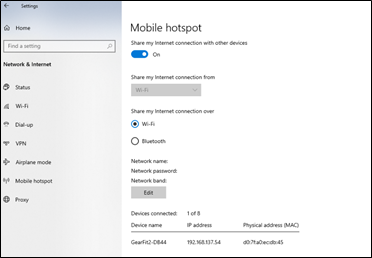
\includegraphics[width=.6\textwidth]{Pic 14.2.png}
\end{center}
  \item Open Tizen, and select “Device Manager” from the Tools tab 
      \begin{center}
    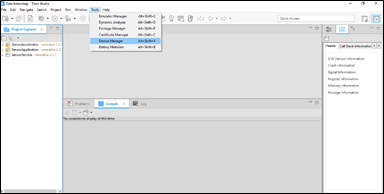
\includegraphics[width=.7\textwidth]{Pic 15.2.png}
\end{center}
  \item When the Device Manager opens, select the “Remote Device Manager”
      \begin{center}
    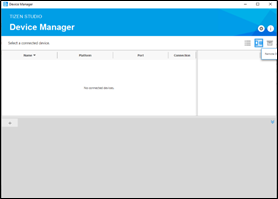
\includegraphics[width=.6\textwidth]{Pic 16.2.png}
\end{center}
  \item In the Remote Device Manager, select the plus sign to connect the watch
      \begin{center}
    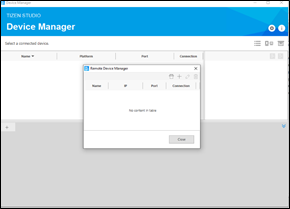
\includegraphics[width=.6\textwidth]{Pic 17.2.png}
\end{center}
  \item Put in Name, and IP address listed in the laptop’s mobile hotspot window 
      \begin{center}
    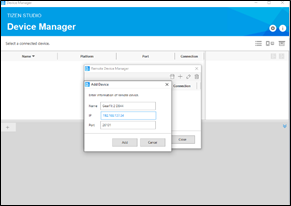
\includegraphics[width=.6\textwidth]{Pic 18.2.png}
\end{center}
\cleardoublepage
  \item Press “Add”, and then turn on the connection, the device information should then appear in the Device Manager
      \begin{center}
    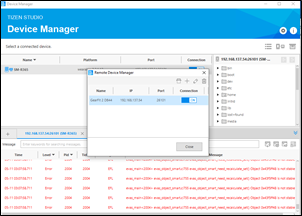
\includegraphics[width=.6\textwidth]{Pic 19.2.png}
\end{center}
\end{enumerate}
\cleardoublepage

\section{Installation of LIACS Sensor App and Sensor Service}
\begin{enumerate}
  \item Make a GitHub account
  \item Ask for an invite to this repository. The current owner is the LiacsProjects organisation run by MarinusVanDijk (m.k.van.dijk@liacs.leidenuniv.nl)
  \item Download from the main branch the software project sensor application and sensor service. Click on "code" and download zip file
  \item Open the project files one by one with the Tizen Studio 4.1
  \item Open the device manager and make connection to the watch
  \item Select the sensor application project, right-click on mouse, choose run-as, choose native device. The software is now downloaded to the watch
  \item Select the sensor service project, right-click on mouse, choose run-as, choose native device
  \item The sensor application is found at the bottom of all applications
  \item Put watch in debug mode, switch all app off with settings only switch on wifi
  \item Push - with the device manager - a configuration file with name ``configuration.dat" on folder ``/opt/var/tmp/". Notes about the configuration file: Write timer can be set to a higher frequency than the data is collected to miss fewer signals The privacy circle has a max range of 5000 mt, anything higher sets the privacy circle to 100 mt
  \item Do a zero measurement (for calibration offline) for 15 minutes, upload the sensor + con files
\end{enumerate}
NOTE: You can also use the sdb (Smart Development Bridge) tool which come with Tizen Studio instead of the Device Manager. (See How to use SDB).

\section{How to Use Smart Development Bridge (SDB)}

The Tizen Studio contains a command prompt tool called ``sdb.exe", the Smart Development Bridge tool. This tool can install packages on the target, as well as pull and push files from and to the target.
https://docs.tizen.org        /application/tizen-studio/common-tools/smart-development-bridge/

\begin{enumerate}
    \item First, after installation of the Tizen Studio environment, copy the sdb.exe from c:/TizenStudio/tools/sdb.exe to c:/Windows/System32 folder
    \item Open a git bash command terminal or windows command prompt
\end{enumerate}
Try the following:

\begin{enumerate}
    \item Get the version number of the smart development bridge
\begin{verbatim}
    $ sdb version
\end{verbatim}
    \item Get the list of all devices connected
    \begin{verbatim}
    $ sdb devices

\end{verbatim}
        \begin{center}
    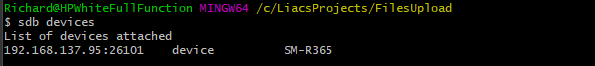
\includegraphics[width=.999\textwidth]{Pic 20.png}
\end{center}
    \item Connect to a device
    \begin{verbatim}
    $ sdb connect 192.168.137.95:26101
\end{verbatim}
    \item Get the ip address
     \begin{verbatim}
    $ sdb get-serialno
\end{verbatim}
        \begin{center}
    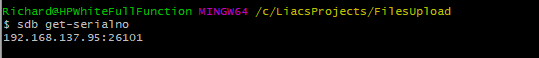
\includegraphics[width=.999\textwidth]{Pic 21.png}
\end{center}
    \item Install a target package on a device
         \begin{verbatim}
    $ sdb install "package name.tpk"
\end{verbatim}
        \begin{center}
    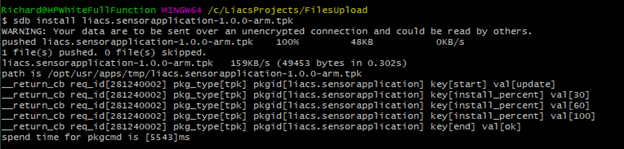
\includegraphics[width=.999\textwidth]{Pic 22.png}
\end{center}
    \item Execute a Linux command on the target
          \begin{verbatim}
   $ sdb shell ls -l opt/var/tmp
\end{verbatim}
       \begin{center}
    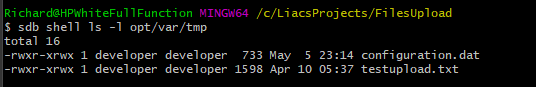
\includegraphics[width=.999\textwidth]{Pic 23.png}
\end{center}
    \item Pull the configuration.dat file from the target
       \begin{verbatim}
   $ sdb pull opt/var/tmp/configuration.dat
\end{verbatim}
      \begin{center}
    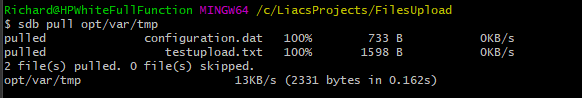
\includegraphics[width=.999\textwidth]{Pic 24.png}
\end{center}
    \item Push the configuration.dat file from the target
       \begin{verbatim}
 $ sdb push opt/var/tmp/configuration.dat
\end{verbatim}
     \begin{center}
    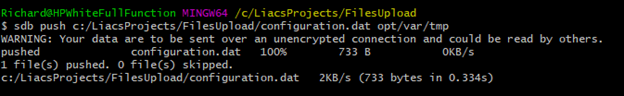
\includegraphics[width=.999\textwidth]{Pic 25.png}
\end{center}
    \item Pull all sensor files from the target
          \begin{verbatim}
$ sdb pull opt/usr/apps/liacs.sensorservice/data
\end{verbatim}
    \begin{center}
    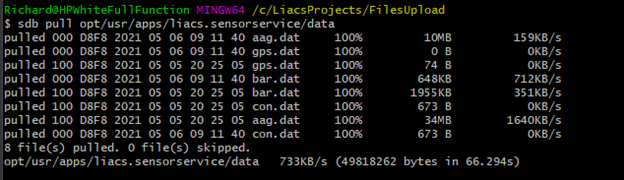
\includegraphics[width=.999\textwidth]{Pic 26.png}
\end{center}
    \item Remove all sensor files from the target
              \begin{verbatim}
$ sdb shell rm opt/usr/apps/liacs.sensorservice/data/*.dat
\end{verbatim}
    \item Disconnect the device
                  \begin{verbatim}
$ sdb disconnect
\end{verbatim}
\end{enumerate}
\cleardoublepage


\section{Possible Errors}
\begin{enumerate}
    \item Tip Windows Installations: In case you cannot run the Device Manager and get a message that msvcr120dll is missing, you will have to load an extension for your OS: 
    \begin{verbatim}
https://answers.microsoft.com/en-us/windows/forum/windows_10-performance
/msvcr120dll-is-missing-or-error/aafe820f-4dbb-4043-aba2-e4ac2dcf69c1
    \end{verbatim}
    \item In case you cannot run the Device Manager and get a message that msvcp120dll is missing, you will have to load an extension for your OS: 
\begin{verbatim}
https://answers.microsoft.com/en-us/windows/forum/windows_7-windows_
install/missing-msvcp120dll-file/f0a14d55-73f0-4a21-879e-1cbacf05e906
\end{verbatim}
\item While uploading the package of the sensor service on another watch, the launch process ends up in an error 75
\begin{verbatim}
"signature invalid device unique id"
\end{verbatim}
\end{enumerate}

Additionally, there are forum questions asked and answered on:


https://wiki.tizen.org/SDK


or more information can be found at:

https://docs.tizen.org/application/tizen-studio/common-tools/certificate-registration/


and at:

https://developer.samsung.com/galaxy-watch-develop             /getting-certificates/create.html


\cleardoublepage
Another hint: In one of the steps in the Certificate Manager you need to    supply is a list of DUID.
    \begin{center}
    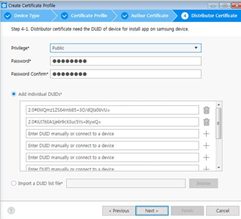
\includegraphics[width=.6\textwidth]{Pic 27.png}
\end{center}

\cleardoublepage
\section{Example Data}
\begin{enumerate}
    \item Activity timeline of gravity accelerometer values with sample frequency of 10 Hz. The first part shows sitting then standing, activity indoors, then sleeping; the watch is on the non-dominant wrist
        \begin{center}
    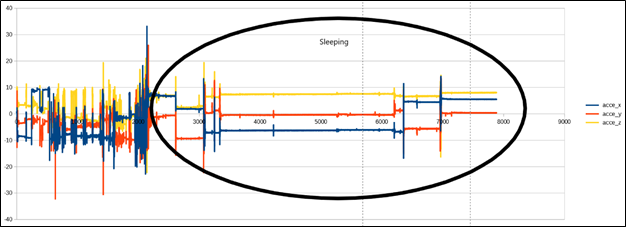
\includegraphics[width=.7\textwidth]{Pic 28.png}
\end{center}
Gyroscope, 10 Hz:
    \begin{center}
    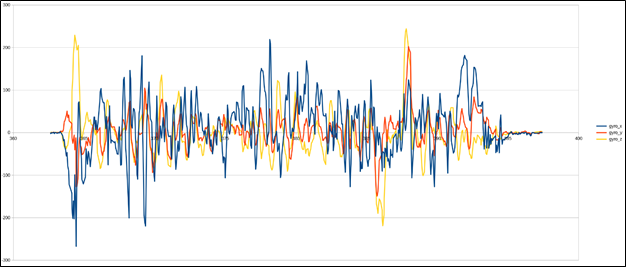
\includegraphics[width=.7\textwidth]{Pic 29.png}
\end{center}
    \item A close-up moment from walking to running:
        \begin{center}
    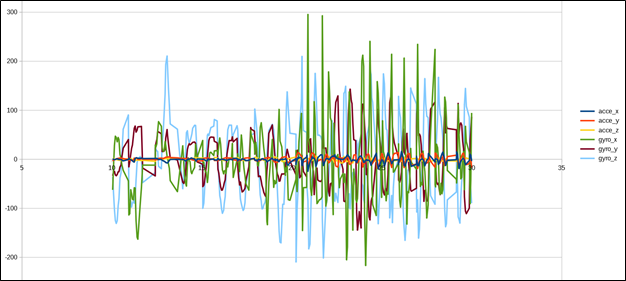
\includegraphics[width=.7\textwidth]{Pic 30.png}
\end{center}
\cleardoublepage
Close-up on sample scale:
    \begin{center}
    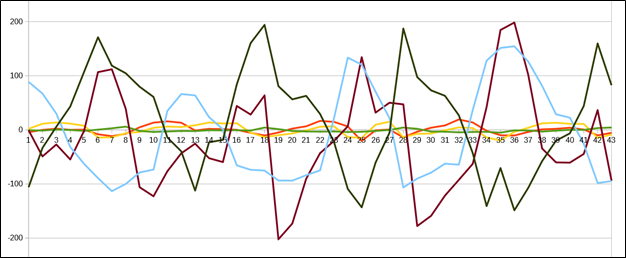
\includegraphics[width=.7\textwidth]{Pic 31.png}
\end{center}
    \item Interval Combination Experiment:
        \begin{center}
    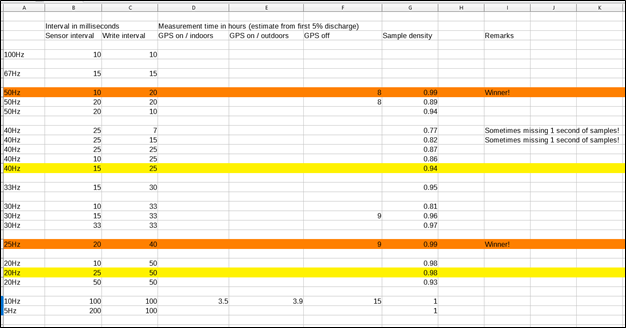
\includegraphics[width=.7\textwidth]{Pic 32.png}
\end{center}
The best combination is 50Hz and 25Hz and lower. For 50Hz take a 10 ms for the sensor intervals and 20 ms for the writer timer interval.
The sample density is a measure calculated by the number of records in the sensor files divided by the time in seconds. This result is divided by the sample frequency expected by the interval settings.
Sample density = number of records / seconds / expected frequency
For example:
For 50Hz the samples expected is 50 per second. 
If the number of records in the sensor file is 4800, the sample density is 4800/5000 = 0.96.
For the best result the sample density must be 1.0

\item Accelerometer 4700 - 5300 seconds:
    \begin{center}
    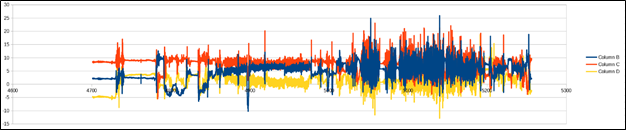
\includegraphics[width=.75\textwidth]{Pic 33.png}
\end{center}
    \begin{center}
    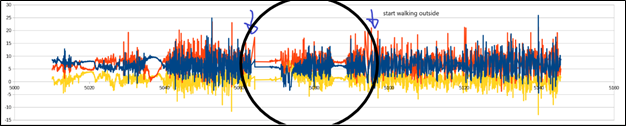
\includegraphics[width=.75\textwidth]{Pic 34.png}
\end{center}
    \begin{center}
    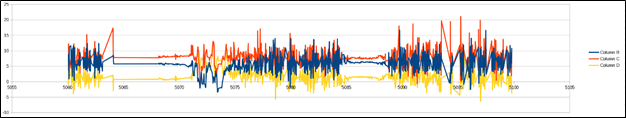
\includegraphics[width=.75\textwidth]{Pic 35.png}
\end{center}
Here there is walking through a door, resting, walking again, resting again, and then stepped out of the building as GPS signal is picked up.
\end{enumerate}
\cleardoublepage
\section{Appendix A}
\title{State Diagram, with transitions and format ``event - actions"}

    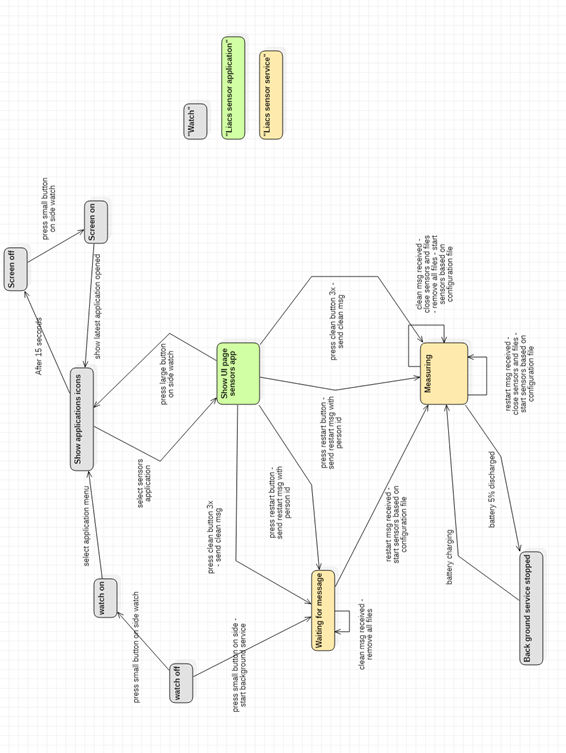
\includegraphics[width=.999\textwidth]{Pic 37.png}
    
\section{Appendix B}
\title{Python Notebook, zero measurement G mean / standard deviation}

\begin{center}
      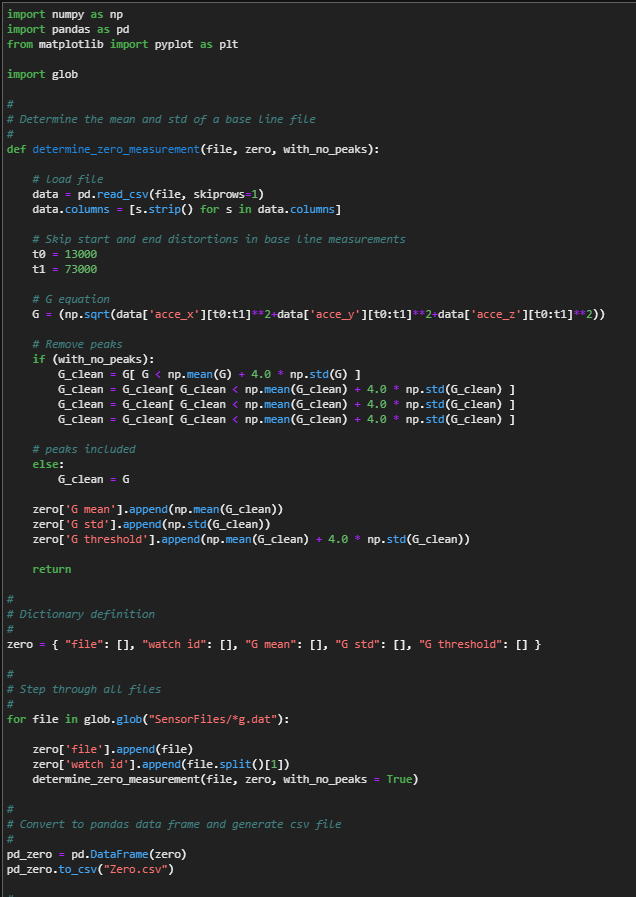
\includegraphics[width=.9\textwidth]{Pic 43.png}  
\end{center}

\section{Appendix C}
\title{Python Notebook, mean and standard deviation plots}

\begin{center}
      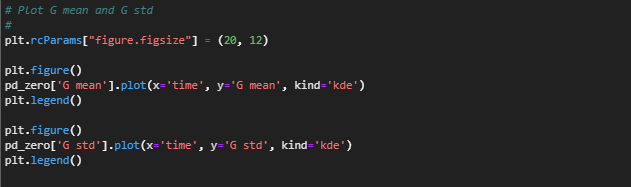
\includegraphics[width=.9\textwidth]{Pic 45.png}  
\end{center}

\begin{center}
      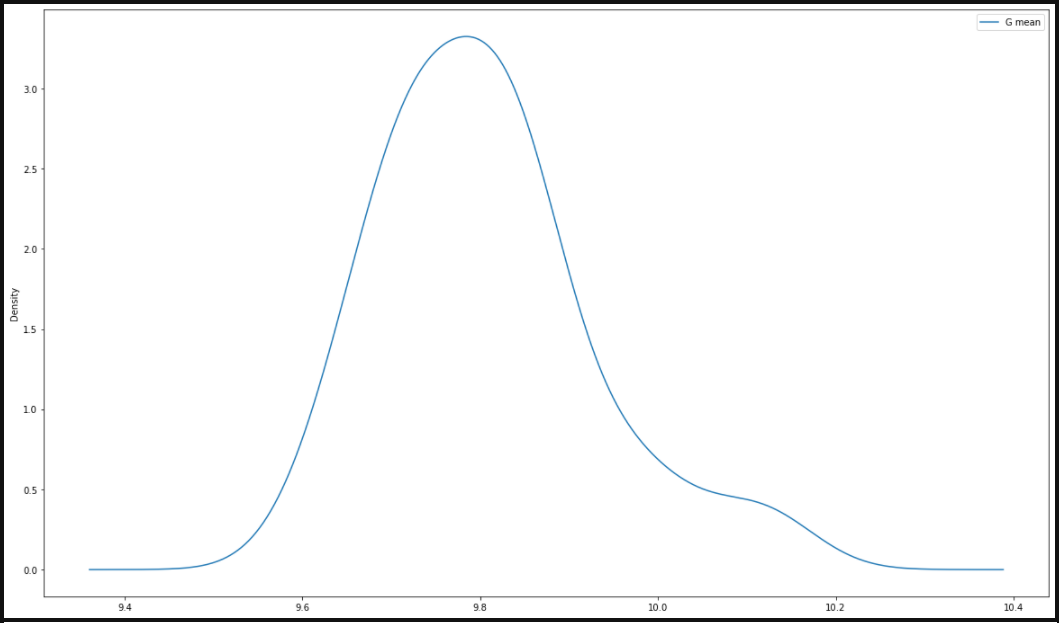
\includegraphics[width=.8\textwidth]{Pic 46.png}  
\end{center}

\begin{center}
      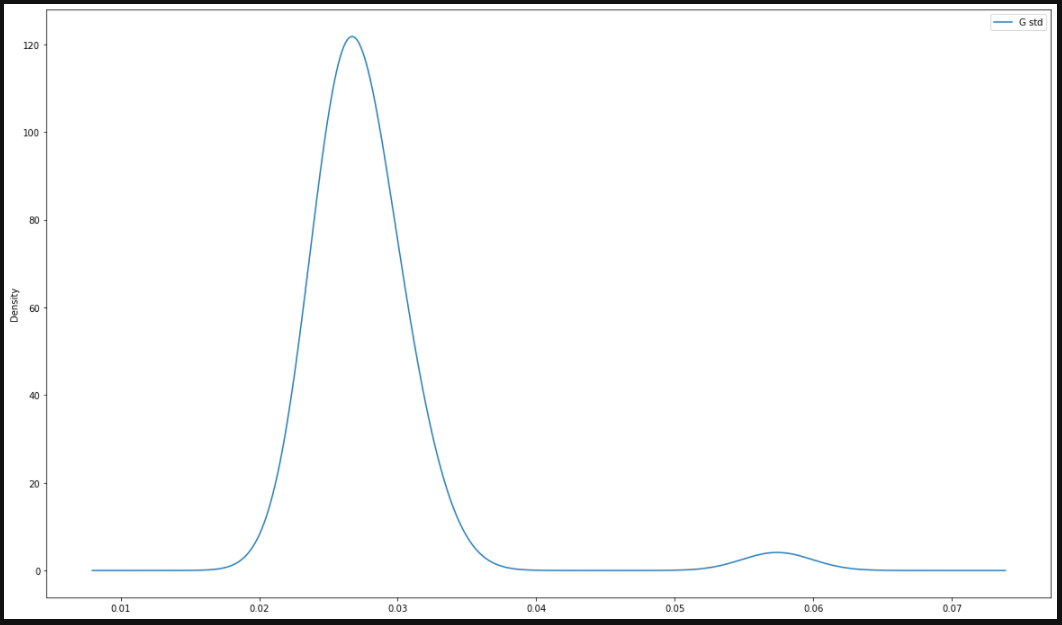
\includegraphics[width=.8\textwidth]{Pic 47.png}  
\end{center}
\end{document}

